\PassOptionsToPackage{colorlinks=true,citecolor=pink,linkcolor=red,urlcolor=cyan}{hyperref}
\documentclass
   [kul] % options: kulak (default) or kul, handout 
   {style/kulakbeamer}

\usepackage{definitions}
\usepackage{svg}
\usepackage[style=apa]{biblatex}
\newcommand{\inner}[2]{\langle #1, #2 \rangle}
\addbibresource{KnotsFractalsReference.bib}

\title{Isometric Immersions of Negatively Curved Metrics}
%\subtitle{Subtitle}
\author[Short name]{Michael McGloin \and (Joeri Van der Veken)} 
\institute{KU Leuven}
%% Overview at the beginning of each section; delete if unwanted.


\begin{document}

\begin{titleframe}
   \vspace{20px}
   % \begin{figure}
   %    \raggedleft
   %    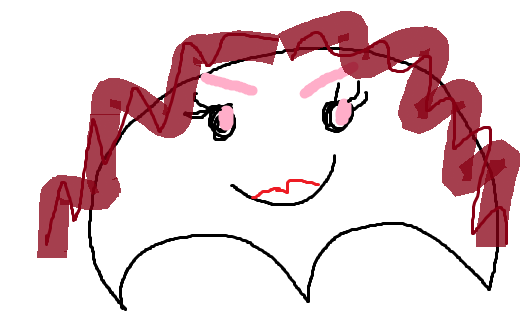
\includegraphics[scale=0.2]{images/image.png}
   % \end{figure}
   \titlepage
\end{titleframe}

\begin{frame}[c]{Hilberts Theorem}
   \begin{kulblock}{Theorem (\cite{Hilbert})}
      There is no isometric immersion of a complete, smooth surface of constant negative curvature into $\mathbb{R}^3$.
   \end{kulblock}\vspace{40px}
   \footnotesize
   \fullcite{Hilbert}

\end{frame}

\begin{frame}{Overview}
   \tableofcontents
\end{frame}

% % % Here you go  % % % 
\section{Hyperbolic Geometry}
\frame[c]{\sectionpage}
\begin{frame}[c]{Euclids Fifth Postulate (Euclid c. 300 BC)}
	\begin{figure}
		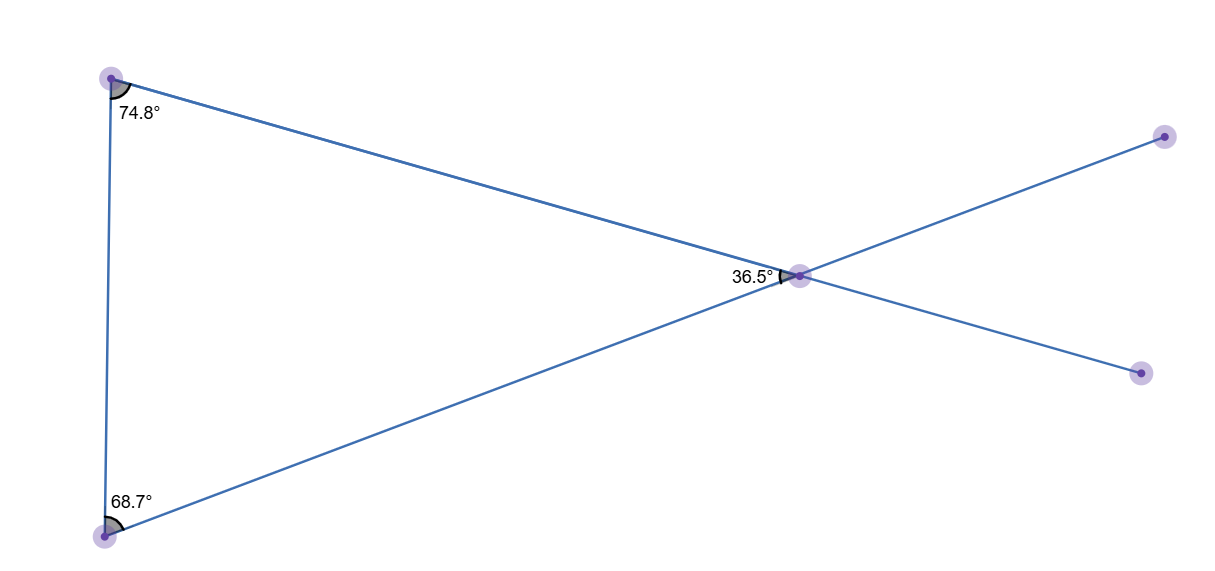
\includegraphics[scale=0.3]{images/Parallel_postulate_en.svg.png}
		\caption{Euclid's 5th postulate}
	\end{figure}
\end{frame}

\begin{frame}[c]{Poincáre Disc Model}
	\begin{figure}
		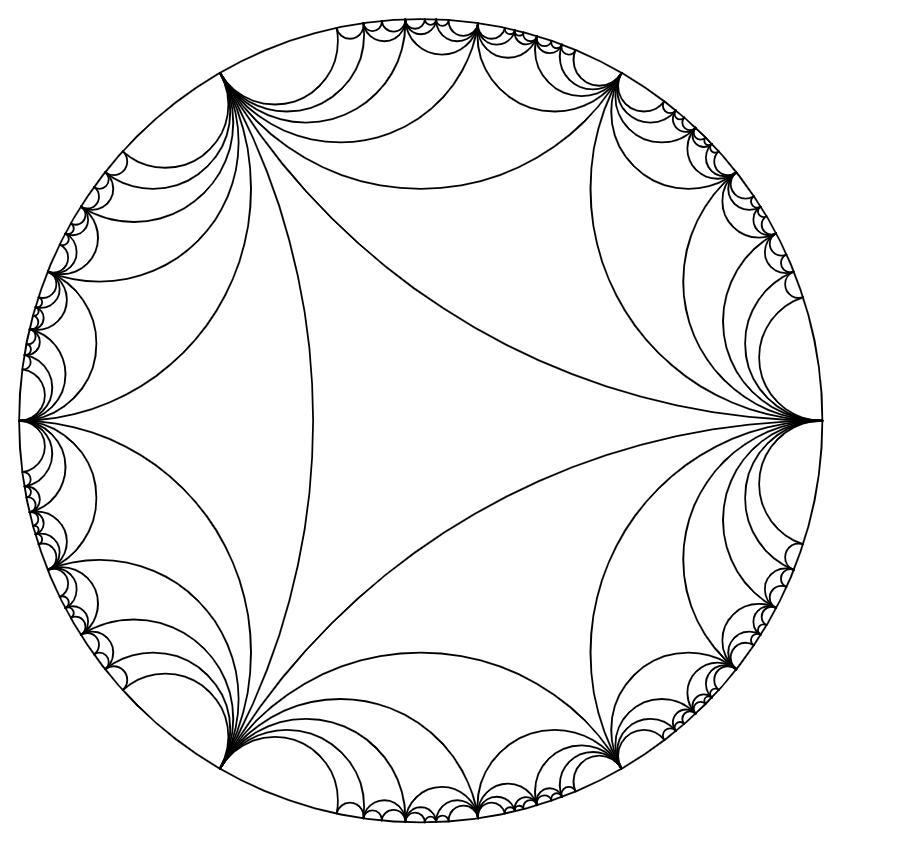
\includegraphics[scale=0.25]{images/PoincaireDisc.png}
		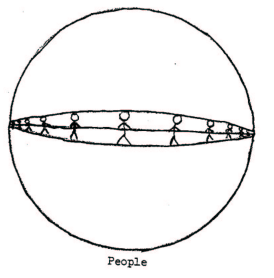
\includegraphics[scale=0.8]{images/PeoplePoincaireDiusc.png}
		\caption{Poincáre Disc Model (\cite{Trott1999Graphica1}) + People on disc (\cite{thurston2022geometry})}
	\end{figure}
\end{frame}

\begin{frame}[c]{Poincáre Half Plane Model}
	\begin{itemize}
		\item Let $\mathbb{H}^2 := \{z \in \mathbb{C} \mid Im(z)>0\}$
	\end{itemize}
	\begin{figure}
		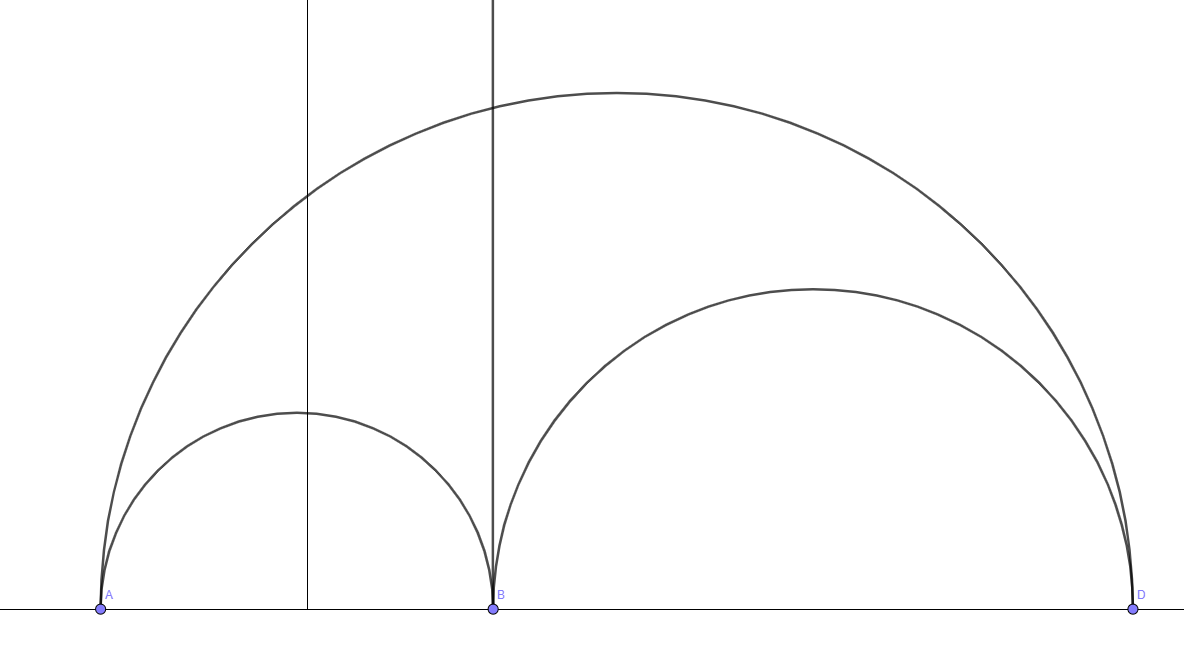
\includegraphics[scale=0.225]{images/hyperbolicdisc.png}
		\caption{Poincáre Half Plane Model}
	\end{figure}
\end{frame}

\begin{frame}[c]{Isometries of the Hyperbolic Plane}
	\begin{itemize}
		\item Isometries are given by elements of $PSL(2, \mathbb{R})$.
	\end{itemize}

	$$\begin{pmatrix}
			a & b \\
			c & d
		\end{pmatrix} \cdot z = \frac{az +b}{cz + d}, \quad a,b,c,d \in \mathbb{R},\hspace{5px} ad-bc = 1$$
\end{frame}

\begin{frame}[c]{Complete Hyperbolic Surfaces}
	\begin{kulblock}{Definition}
		A (hyperbolic) surface is \emph{complete} if its straight lines can be continued indefinitely.
	\end{kulblock}
	\pause
	\begin{kulblock}{Theorem (\cite{Hopf1926CliffordKlein}, \cite{Killing1891CliffordKlein})}
		Any complete hyperbolic surface is the quotient $\mathbb{H}^2/\Gamma$ where $\Gamma$ is a discrete subgroup of $PSL(2, \mathbb{R})$. These groups are called \emph{Fuschian groups}.
	\end{kulblock}
\end{frame}

\begin{frame}[c]{Complete Hyperbolic Surfaces}
	\begin{figure}
		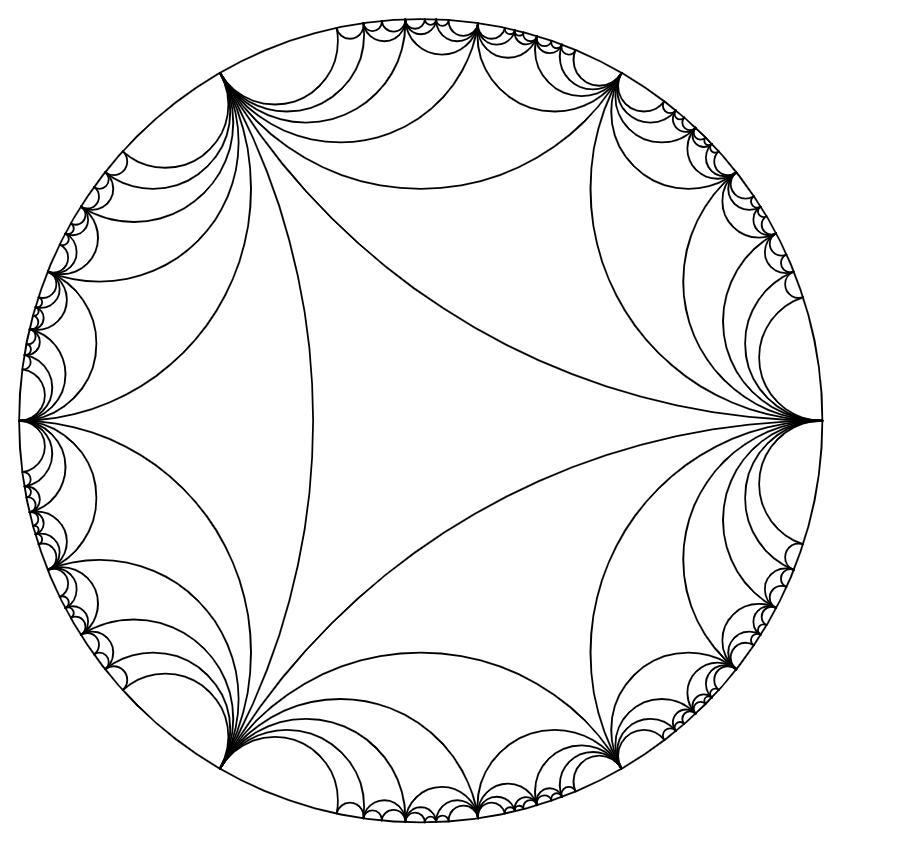
\includegraphics[scale=0.25]{images/PoincaireDisc.png}
		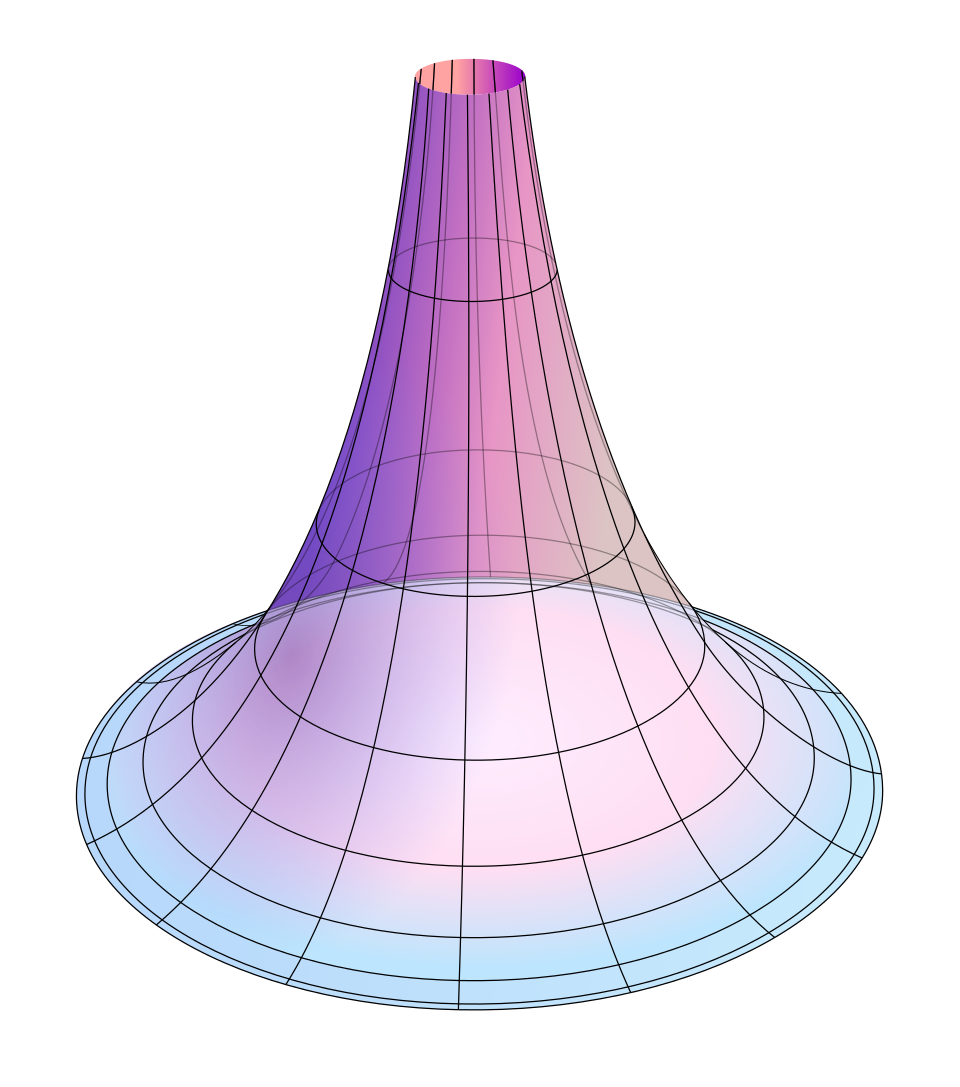
\includegraphics[scale=0.15]{images/PseudoSphere.svg.png}
		\caption{Poincaire Disc Model (\cite{Trott1999Graphica1})  and the Pseudo-sphere (WikiCommons)}
	\end{figure}
\end{frame}

\section{Curvature}
\frame[c]{\sectionpage}

\begin{frame}[c]{Curvature}
	\begin{center}
		\Large{What is curvature?}
	\end{center}
\end{frame}

\begin{frame}[c]{Curvature}
	\begin{figure}
		\centering
		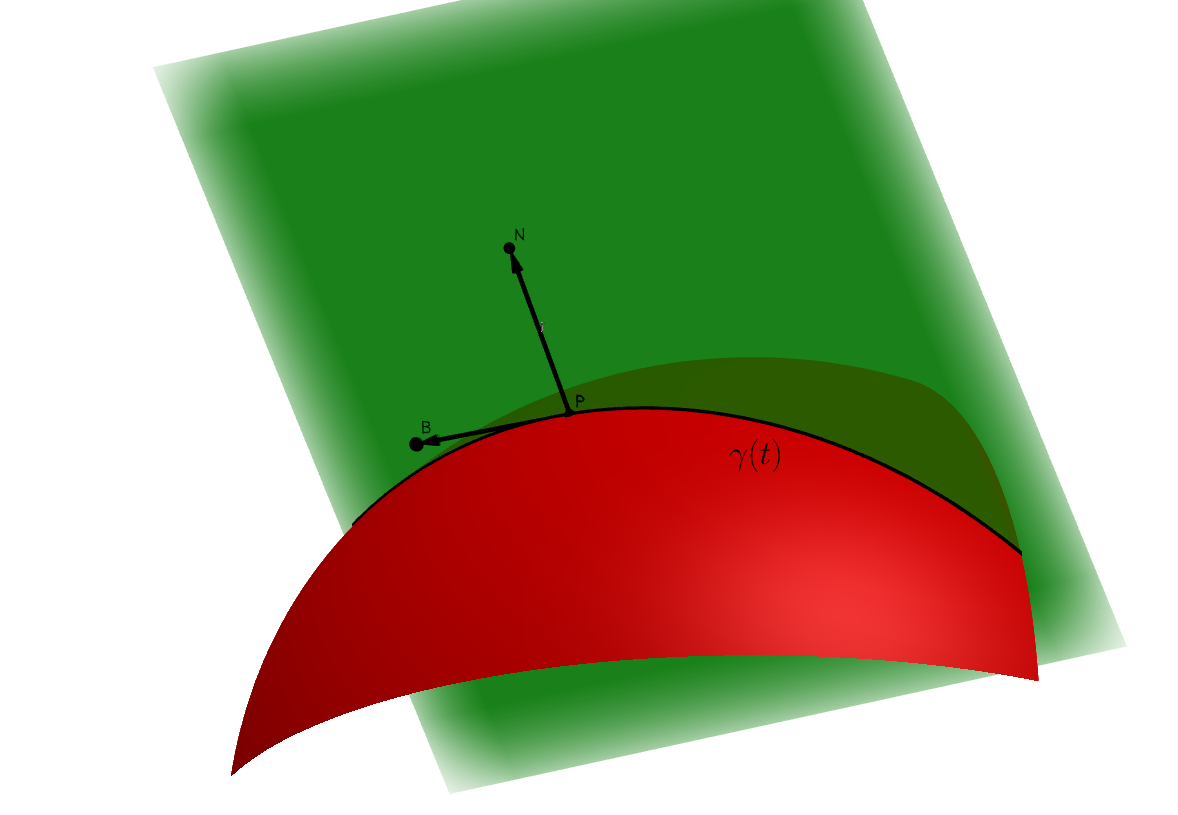
\includegraphics[scale=0.25]{images/Normal to the Surface.png}
		\caption{Normal section of a curved surface}
	\end{figure}
\end{frame}

\begin{frame}[c]{Fundamental Pair}
	\begin{kulblock}{Definition}
		A \emph{fundamental pair} on a manifold $M$ is a pair $(I,II)$ of symmetric, bilinear forms defined on $TM$ such that $I$ is a metric.
	\end{kulblock}
	\pause
	In coordinates, $$I = \begin{pmatrix}
			E & F \\ F & G
		\end{pmatrix}, \quad II = \begin{pmatrix}
			e & f \\ f & g
		\end{pmatrix}$$
	\pause
	\begin{definition}
		The shape operator $S$ is defined by $I(SX, Y) = II(X,Y)$. In coordinates $S = I^{-1}II$
	\end{definition}
\end{frame}

\begin{frame}[c]{Curvature of a Fundamental Pair}
	\begin{kulblock}{Definition}
		The \emph{extrinsic} curvature $K$ of a fundamental pair $(I, II)$, is defined to be
		$$K = \dfrac{eg-f^2}{EG- F^2} = \kappa_1 \kappa_2 = \det (S)$$
		where $\kappa_1, \kappa_2$ are the eigenvalues (principal curvatures) of $S$.
	\end{kulblock}
\end{frame}

\begin{frame}[c]{This is Intrinsic!}
	\begin{kulblock}{Theorem Egregium (Gauss 1827)}
		\begin{center}
			Let $(I, II)$ be the canonical fundamental pair associated to a surface in $\mathbb{R}^3$. Then the quantity $K = \kappa_1 \kappa_2$ is intrinsic!
		\end{center}
	\end{kulblock}
	\begin{figure}
		\centering
		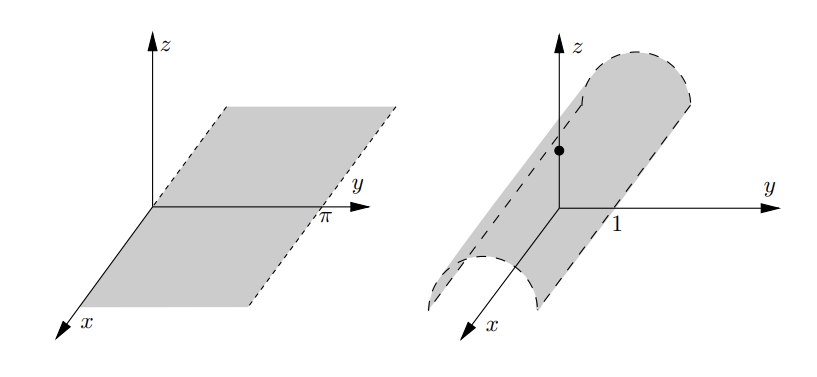
\includegraphics[scale=0.3]{images/intrinsicillustratyion.png}
		\caption{Two isometric surfaces with different principle curvatures (Lee)}
	\end{figure}
\end{frame}

\begin{frame}[c]
	\begin{center}
		\Large{What about surfaces not in $\mathbb{R}^3?$}
	\end{center}
\end{frame}

\begin{frame}[c]{Riemannian Manifolds and Isometric Immersion}
	\begin{kulblock}{Definition}
		A manifold $M$ is Riemannian if there is an inner product $\inner{\cdot}{\cdot}$ defined on each tangent space and $\inner{\cdot}{\cdot}$ varies smoothly.
	\end{kulblock}
	\pause
	\begin{kulblock}{Definition}
		An isometric immersion $$\varphi:(M,\inner{\cdot}{\cdot}_1) \to (N, \inner{\cdot}{\cdot}_2)$$
		is a smooth, distance preserving map such that $d\varphi$ is injective everywhere.
	\end{kulblock}
\end{frame}

\begin{frame}[c]{Connections}

	\begin{kulblock}{Definition}
		Let $(M , \inner{\cdot}{\cdot})$ be a Riemannian manifold. A connection on the tangent bundle $TM$ is a map
		$$ \nabla : \text{Vect}(M) \times \text{Vect}(M) \to \text{Vect}(M)$$
		that satisfies $\nabla_X fY = X(f)Y + f\nabla_XY$ for $f \in C^{\infty}(M)$ and otherwise is linear.
	\end{kulblock}
	\begin{remark}
		There is a canonical connection associated to a Riemannian manifold called the \emph{Levi Civita} connection. (\cite{Lee})
	\end{remark}
\end{frame}

\begin{frame}[c]{Riemann Curvature Tensor}
	\begin{kulblock}{Definition}
		Let $(M,\inner{\cdot}{\cdot})$ be a Riemannian manifold. The Riemann curvature tensor is defined as
		$$ R(X,Y)Z = \nabla_X \nabla_Y Z - \nabla_Y \nabla_X Z - \nabla_{[X,Y]} Z$$
	\end{kulblock}
	\begin{kulblock}{Definition}
		The \emph{sectional curvature} of $\Pi =\text{span}(e_1,e_2) \subset T_pM$ is defined as
		$$sec(\Pi) = \langle R(e_1, e_2)e_1, e_2 \rangle$$
	\end{kulblock}
\end{frame}

\begin{frame}[c]{Space Forms}
	\begin{kulblock}{Definition}
		A \emph{space form} is a complete Riemannian manifold $M$ with constant sectional curvature.
	\end{kulblock}
	\pause
	\begin{remark}
		If $M$ is a complete simply connected Riemannian manifold with constant sectional curvature $c$
		\begin{itemize}
			\item $c=0 \implies M \cong \mathbb{R}^n$
			\item $c = 1 \implies M \cong S^n$
			\item $ c = -1 \implies M \cong \mathbb{H}^n$
		\end{itemize}
	\end{remark}
\end{frame}

\section{Codazzi Pairs}
\frame[c]{\sectionpage}
\begin{frame}[c]{Gauss Equation}
	Let $\mathbb{M}^3(c)$ denote the unique simply connected space form with sectional curvature $c$ and $\Sigma$ be a surface.
	\pause
	\begin{kulblock}{Theorem}
		The Gauss equation of an immersion $f: (\Sigma,I) \to \mathbb{M}^3(c)$ is given by
		$$K(I) = K + c$$
		where $K = \det(S)$ is the extrinsic curvature and $K(I)$ is the intrinsic curvature e.g. the sectional curvature $sec(T_p\Sigma)$.
	\end{kulblock}
\end{frame}

\begin{frame}[c]{Codazzi Pair}
	\begin{kulblock}{Definition}
		A fundamental pair $(I, II)$ with shape operator $S$ is a Codazzi pair if the Codazzi equation is satisfied - i.e.
		$$\nabla_X SY - \nabla_Y SX - S[X, Y] = 0$$
		for $X,Y \in \text{Vec}(\Sigma)$ and $\nabla$ is the induced Levi-Civita connection on $\Sigma$.
	\end{kulblock}
\end{frame}

\section{Hilberts Theorem}
\frame[c]{\sectionpage}
\begin{frame}[c]{Asymptotic Curves}
	\begin{kulblock}{Definition}
		An asymptotic direction $v\in T_p \Sigma$ on $\Sigma$, is a direction where $II_p(v,v) = 0$. If $K<0$ at $p\in \Sigma$ there are two asymptotic directions.
	\end{kulblock}
	\begin{figure}
		\centering
		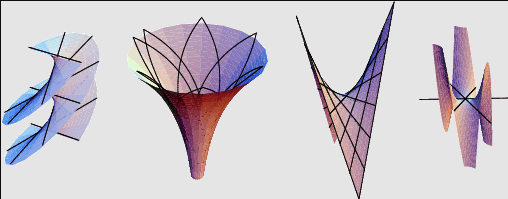
\includegraphics[scale=0.5]{images/asymptoticcurves.png}
		\caption{Asymptotic curves on some surfaces for the second fundamental form. (Wolfram)}
	\end{figure}
\end{frame}

\begin{frame}[c]{Arc Length Paramaterization}
	\begin{kulblock}{Proposition (\cite{firstarticle})}
		Let $(I,II)$ be a Codazzi pair on an oriented, simply connected surface of negative constant extrinsic curvature $K$. Then in local coordinates $(u,v)$ we can write $(I, II)$ as
		$$I =\begin{pmatrix}
				1           & \cos \omega \\
				\cos \omega & 1
			\end{pmatrix}, \quad II = \begin{pmatrix}
				0                    & \sqrt{-K}\sin \omega \\
				\sqrt{-K}\sin \omega & 0
			\end{pmatrix}$$
		with $0<\omega < \pi$.
	\end{kulblock}
\end{frame}

\begin{frame}[c]{Change of Coordinates}
	Paramaterizing by curves $(u,v)$ along the asymptotic directions
	\begin{center}
		$I = \begin{pmatrix}
				E & F \\ F & G
			\end{pmatrix}, \quad$ $II = \begin{pmatrix}
				0 & f \\ f & 0
			\end{pmatrix}, \quad f> 0$
	\end{center}
	\pause
	\begin{itemize}
		\item<2-> If $\dfrac{\partial E}{\partial v} = \dfrac{\partial G}{\partial u} = 0$ then
		      we can paramaterize by arc length as $E = E(u)$ and $G = G(v)$
		\item<3-> This will hold true if $\nabla_{\frac{\partial}{\partial u}}
			      \frac{\partial}{\partial v} = \nabla_{\frac{\partial}{\partial v}}
			      \frac{\partial}{\partial u} = 0 $
	\end{itemize}
	\uncover<4->{
		\begin{remark}
			Recall $\nabla_{\frac{\partial}{\partial u}}
				\frac{\partial}{\partial v} = \nabla_{\frac{\partial}{\partial v}}
				\frac{\partial}{\partial u} = \Gamma_{12}^1  \frac{\partial}{\partial u} + \Gamma_{12}^2  \frac{\partial}{\partial v}$
		\end{remark}}
\end{frame}

\begin{frame}[c]{Can we parametrize nicely?}
	Letting $D = EG - F^2$ we can calculate the following conditions on the Christoffel symbols using Koszul's formula
	\begin{align}
		\frac{D_u}{2D} = \Gamma_{11}^1 + \Gamma_{12}^2, \quad \frac{D_v}{2D} = \Gamma_{22}^2 + \Gamma_{12}^1
	\end{align}
	\pause
	Now using the Codazzi equation we get the following condition on the Christoffel symbols
	\begin{align}
		\frac{f_u}{f} = \Gamma_{11}^1 - \Gamma_{12}^2, \quad \frac{f_v}{f} = \Gamma_{22}^2 - \Gamma_{12}^1
	\end{align}
\end{frame}

\begin{frame}[c]{Can we parametrize nicely?}
	Subtracting the corresponding equations of $(1) - (2)$ we obtain
	\begin{align}
		\frac{f_u}{f} - \frac{D_u}{2D}= 2\Gamma_{12}^2, \quad \frac{D_v}{2D} - \frac{f_v}{f} = 2\Gamma_{12}^1
	\end{align}
	\pause
	We now have that $K = -\dfrac{f^2}{D}$ is a negative constant $\implies K_u =
		K_v =0$.
	\begin{remark}
		These derivatives give exactly the numerator of the LHS and RHS respectively and so
		$\Gamma_{12}^2 = \Gamma_{12}^1 = 0$
	\end{remark}
\end{frame}

\begin{frame}[c]{Arc Length Paramaterization}
	\begin{kulblock}{Proposition (\cite{firstarticle})}
		Since $E(u,v) = E(u)$ and $G(u,v) = G(v)$ we can parametrize locally by arc length and write our Codazzi pair as
		$$I = \begin{pmatrix}
				1           & \cos \omega \\
				\cos \omega & 1
			\end{pmatrix}, \quad II = \begin{pmatrix}
				0                     & \sqrt{-K}\sin \omega \\
				\sqrt{-K} \sin \omega & 0
			\end{pmatrix}$$
		with $0<\omega < \pi$ as $1-F^2 >0$.
	\end{kulblock}
	\begin{proof}
		$K = -\dfrac{f^2}{1-F^2} \implies F^2 + \left(\dfrac{f}{\sqrt{-K}}\right)^2 = 1$
	\end{proof}
\end{frame}

\begin{frame}[c]{We have a global diffeomorphism!}
	\begin{kulblock}{Proposition (\cite{firstarticle})}
		The map $ (u,v) : \Sigma \to \mathbb{R}^2$ is a global diffeomorphism e.g. our coordinates are global.
	\end{kulblock}
	\begin{proof}
		Let $III = du^2 - 2 \cos \omega dudv + dv^2$. Then $I + III = 2(du^2+dv^2)$ is a complete flat metric when $I$ is complete and
		$$ (u,v) : (\Sigma, du^2 + dv^2) \to \mathbb{R}^2$$
		is a local isometry, hence a covering map by completeness and hence a global diffeomorphism by simply connectedness.
	\end{proof}
	% \url{http://staff.ustc.edu.cn/~spliu/HuZhangZhao.pdf} theorem 2.10
\end{frame}

\begin{frame}[c]{Hilberts Theorem}
	\begin{kulblock}{Theorem (\cite{Hilbert}, \cite{firstarticle})}
		Let $\Sigma$ be a complete surface of constant negative Gauss curvature $K(I)$. Then there is no isometric immersion
		$$ f : \Sigma \to \mathbb{M}^3(c)$$
		for $c=0,1$ and if $c = -1$ there is no such immersion if $K(I) < -1$.
	\end{kulblock}
\end{frame}

\begin{frame}[c]{Hilberts Theorem Proof}
	\begin{proof}
		By our first theorem we can find global coordinates $(u, v)$ defined in $\mathbb{R}^2$ such that
		$$I =\begin{pmatrix}
				1           & \cos \omega \\
				\cos \omega & 1
			\end{pmatrix}, \quad II = \begin{pmatrix}
				0                    & \sqrt{-K}\sin \omega \\
				\sqrt{-K}\sin \omega & 0
			\end{pmatrix}$$
		and $0< \omega < \pi$. The Gauss equation \emph{requires} that
		$$\frac{\partial}{\partial v}\omega_{u} = -(K+c)\sin \omega$$
		where $-(K+ c) > 0$.
	\end{proof}
\end{frame}

\section{Extensions of Hilberts Theorem}
\frame[c]{\sectionpage}

\begin{frame}[c]{Non-constant negative curvature}
	\begin{kulblock}{Theorem (Efimov 1963)}
		Let $\Sigma$ be a complete surface with Gauss curvature $K(I) \leq \delta < 0$. Then there is no isometric immersion
		$$ f : \Sigma \to \mathbb{R}^3$$.
	\end{kulblock}
\end{frame}

\begin{frame}[c]{Strictly Seperated Curvatures}
	\begin{kulblock}{Definition}
		The principle curvatures, $\kappa_1,\kappa_2$, of a fundamental pair $(I, II)$ are called \emph{strictly separated} if there exists numbers $c_1,c_2$ such that
		$$\kappa_1 \leq c_1 < c_2  \leq \kappa_2$$
	\end{kulblock}
\end{frame}

\begin{frame}[c]{Non-constant negative curvature}
	\begin{kulblock}{Theorem (\cite{GALVEZ20151058})}
		Let $(I,II)$ be a Codazzi pair on $\Sigma$ with strictly separated principal curvatures. If $(\Sigma, I)$ is a
		complete surface with Gauss curvature $K(I) \leq 0$ and $I$ is not flat then $\Sigma$ is homeomorphic to a plane. \\

		Furthermore, $$\int_{\Sigma}^{} |K(I)|dA \leq 2 \pi$$ where $dA$ is the area
		form induced by $I$.
	\end{kulblock}
\end{frame}

\begin{frame}[c]{Non-constant negative curvature}
	\begin{kulblock}{Corollary (\cite{GALVEZ20151058})}
		Let $\varphi: \Sigma \to \mathbb{H}^3$ be an immersion with Gaussian curvature $K(I) \leq -1$, and one of its principle curvature functions satisfying
		$$\kappa_i \geq \epsilon > 0, \quad \text{for } \epsilon>0 $$
		then $\varphi$ is not a complete immersion.
	\end{kulblock}
\end{frame}

\begin{frame}[c]{Questions?}
	\begin{center}
		\Large{Questions?}
	\end{center}

\end{frame}
\begin{frame}[allowframebreaks]{References}
   \printbibliography
\end{frame}
\end{document}